\documentclass[informe.tex]{subfiles}
\begin{document}
  
  \section{Resultados}
  
    Uno de los primeros experimentos realizados fue variar la cantidad de neuronas en una sola capa oculta para cada problema considerando las cantidades de épocas mencionadas anteriormente. A continuación presentamos resultados sobre dichos experimentos.
    
    
    \begin{figure}[H]
      \begin{center}
	  \hspace*{-2cm}
	  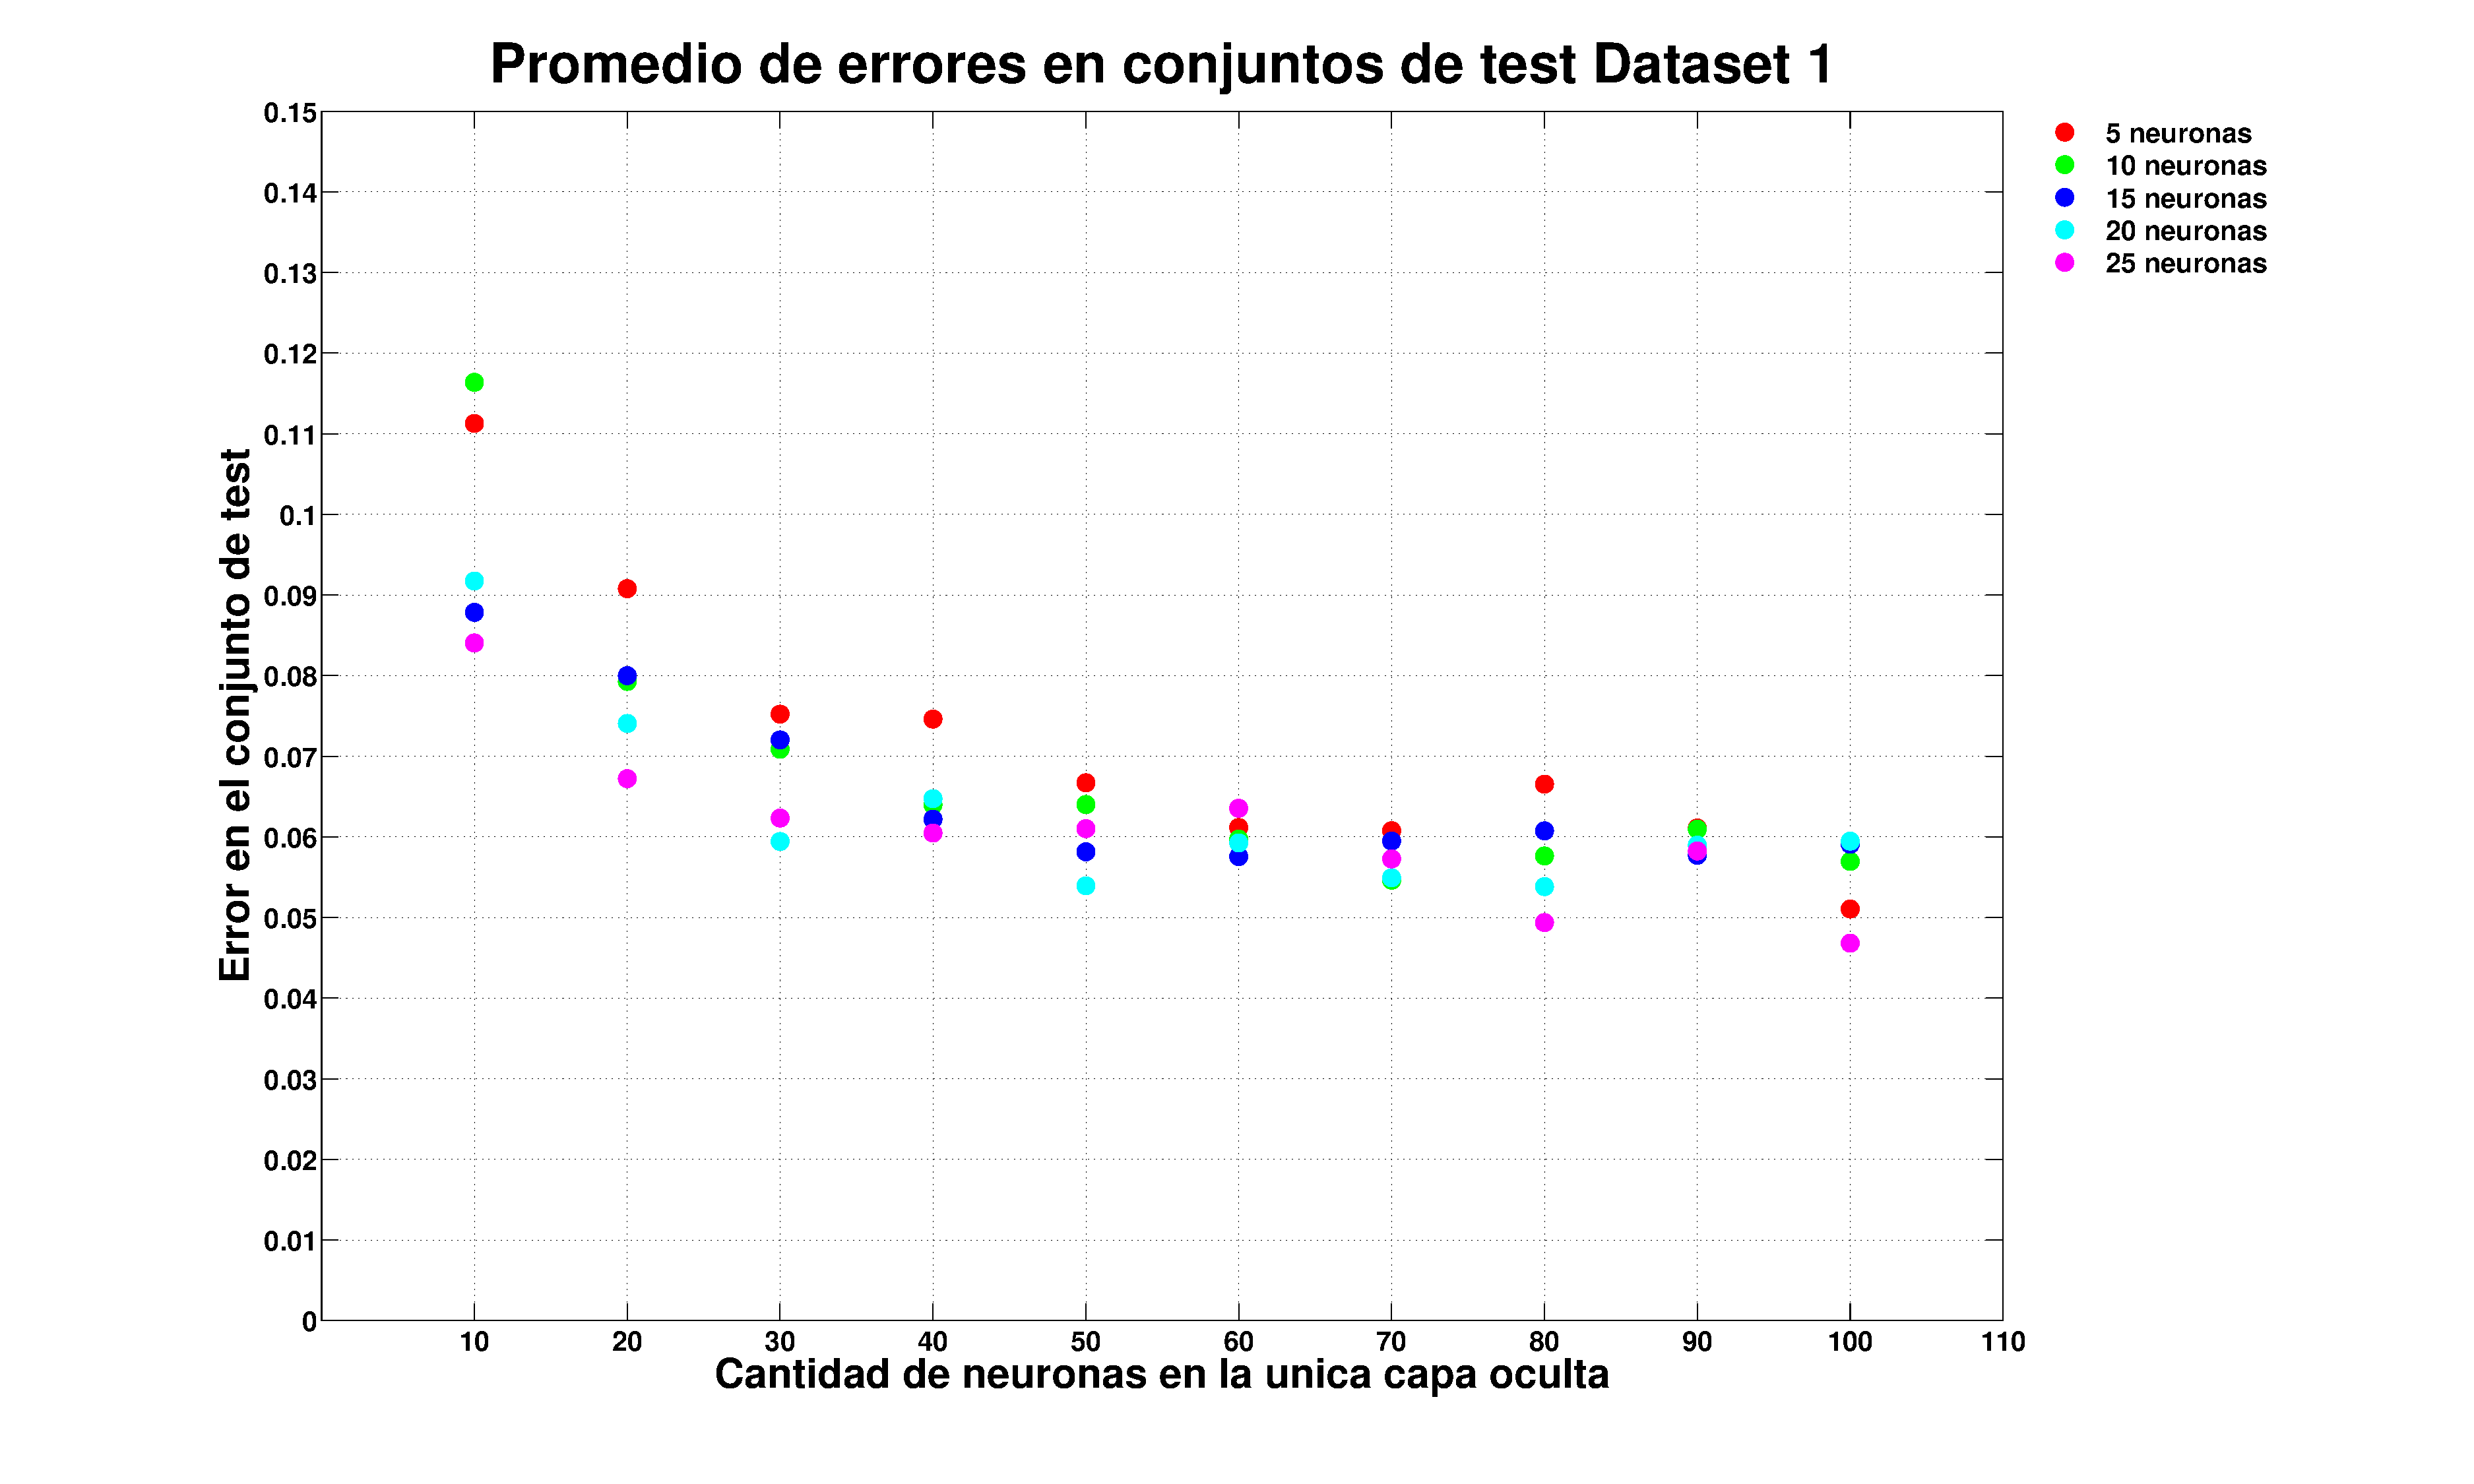
\includegraphics[width=20cm]{graficos/d1_01.pdf}
	  \caption{Promedio de error entre los 4 folds para el dataset 1 calculado sobre el conjunto de test usando $\gamma=0.1$}
	  \label{fig:errorTest-d1}
      \end{center}
    \end{figure}

    \begin{figure}[H]
      \begin{center}
	  \hspace*{-2cm}
	  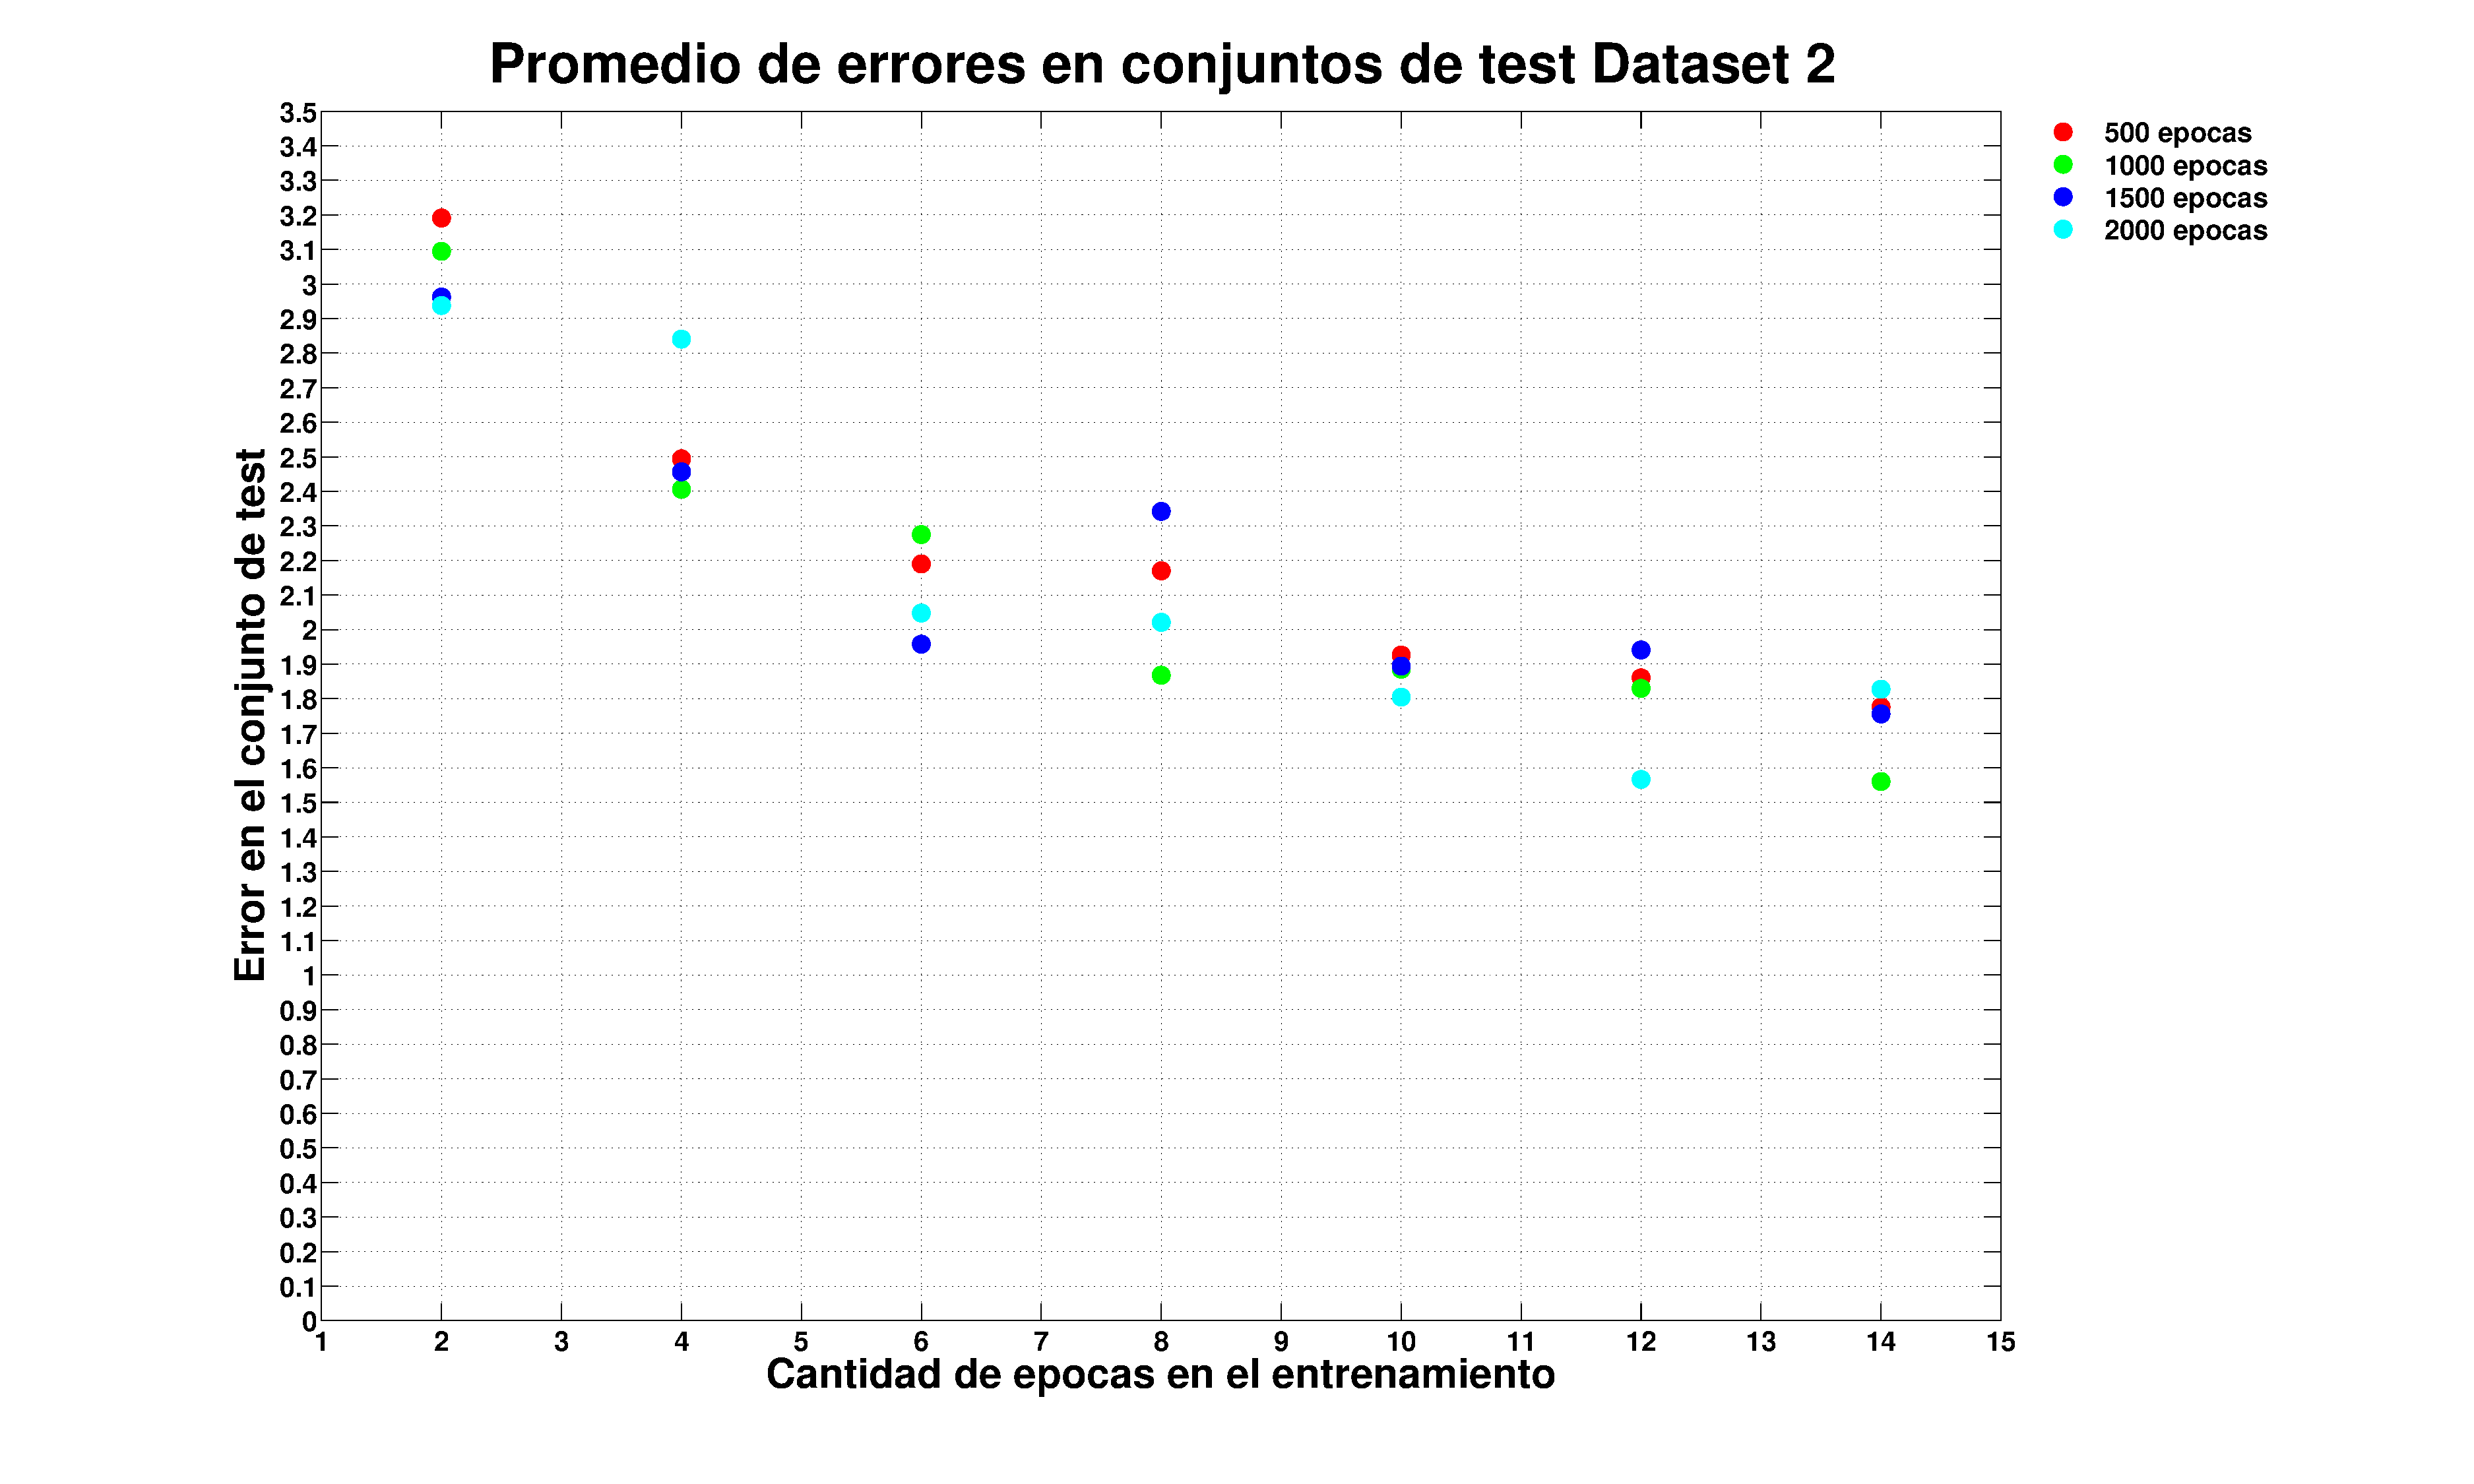
\includegraphics[width=20cm]{graficos/d2_01.pdf}
	  \caption{Promedio de error entre los 4 folds para el dataset 2 calculado sobre el conjunto de test usando $\gamma=0.1$}
	  \label{fig:errorTest-d2}
      \end{center}
    \end{figure}
    
    
    \subsection{Problema 1}
      
      Dado que según la Figura \ref{fig:errorTest-d1} las configuraciones con 5 y 10 neuronas no presentan tan buenos resultados, mostramos a continuación (Figura \ref{fig:p1-f1-gamma01}) gráficos sobre la convergencia del error en función de las épocas usando las otras arquitecturas evaluadas. Para ello mostramos el fold 1 pero los demás presentan un comportamiento similar.
      
      \begin{figure}[H]
        \centering
        \begin{subfigure}[b]{0.32\textwidth}
                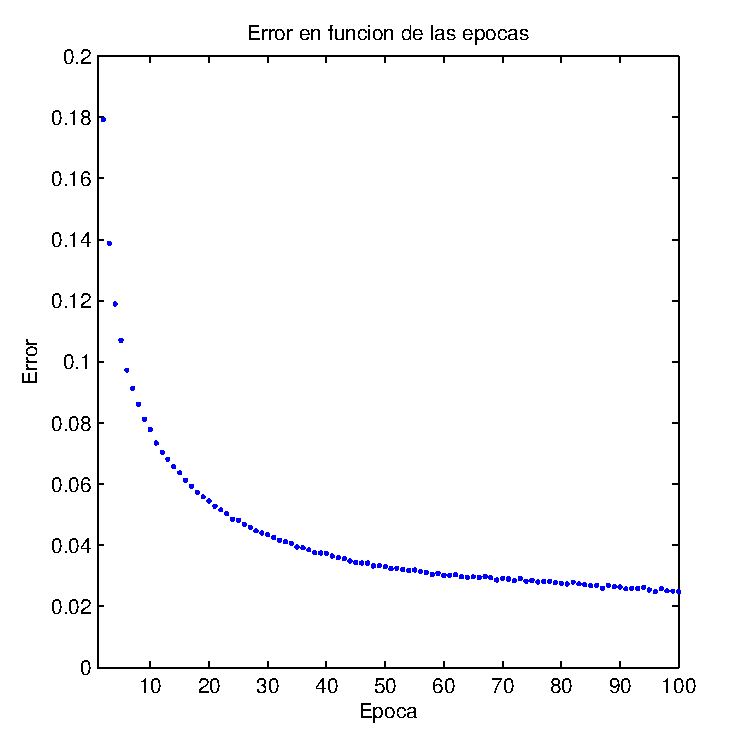
\includegraphics[width=\textwidth]{graficos/error_fold1_15_binary_100_01.pdf}
                \caption{Usando 15 neuronas.}
                \label{fig:d1-f1-01-n15}
        \end{subfigure}
        \begin{subfigure}[b]{0.32\textwidth}
                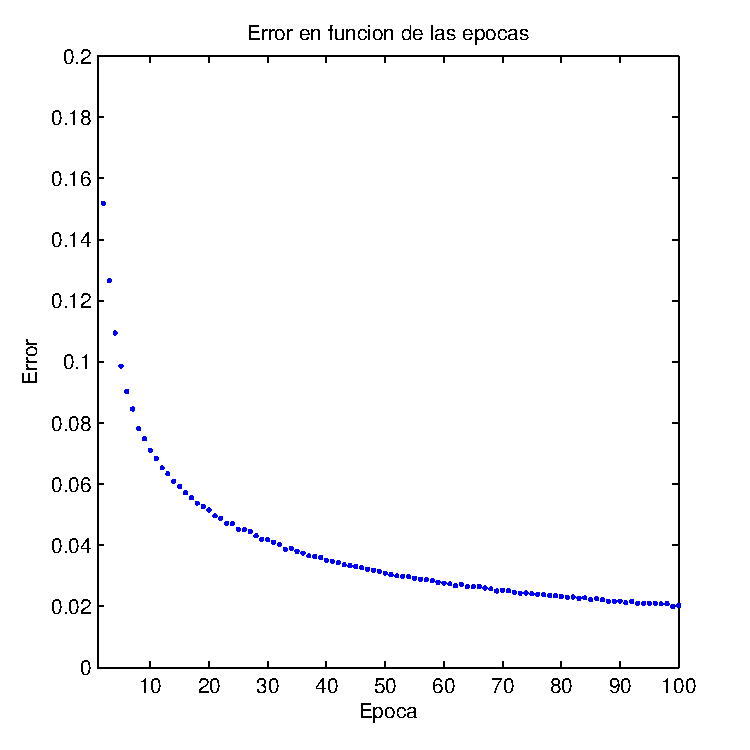
\includegraphics[width=\textwidth]{graficos/error_fold1_20_binary_100_01.pdf}
                \caption{Usando 20 neuronas.}
                \label{fig:d1-f1-01-n20}
        \end{subfigure}
        \begin{subfigure}[b]{0.32\textwidth}
                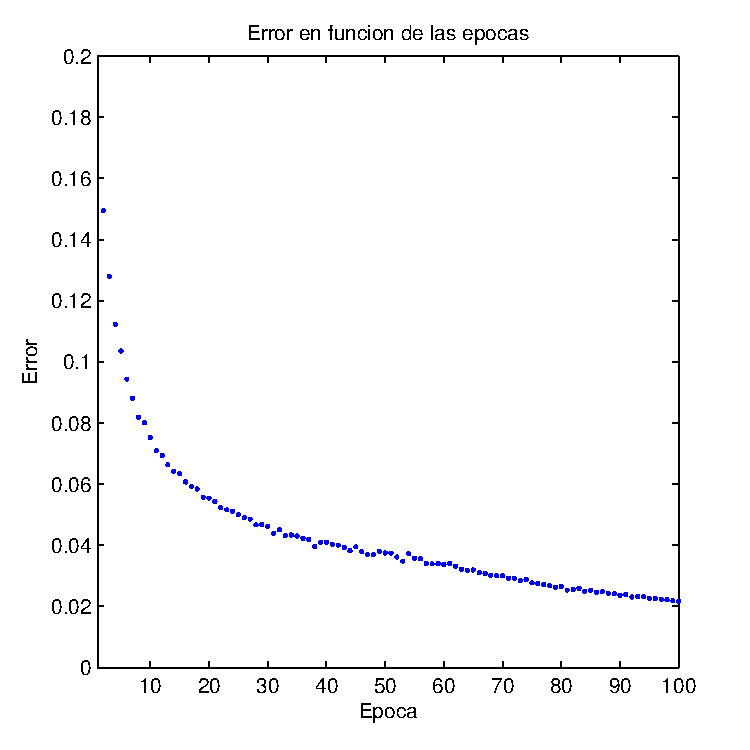
\includegraphics[width=\textwidth]{graficos/error_fold1_25_binary_100_01.pdf}
                \caption{Usando 25 neuronas.}
                \label{fig:d1-f1-01-n25}
        \end{subfigure}
        
        \caption{Error durante el entrenamiento en el fold 1 del problema 1 usando una sola capa oculta y $\gamma=0.1$.}\label{fig:p1-f1-gamma01}
    \end{figure}
    
    Considerando esos resultados, decidimos analizar qué sucedía al utilizar valores de $\gamma$ mayores ya que tal vez era posible converger más rápidamente. Los resultados se encuentran en las Figuras \ref{fig:p1-f1-gamma02}, \ref{fig:p1-f1-gamma03}, \ref{fig:p1-f1-gamma04} y \ref{fig:p1-f1-gamma05}, nuevamente para 15, 20 y 25 neuronas.
    
    \begin{figure}[H]
        \centering
        \begin{subfigure}[b]{0.32\textwidth}
                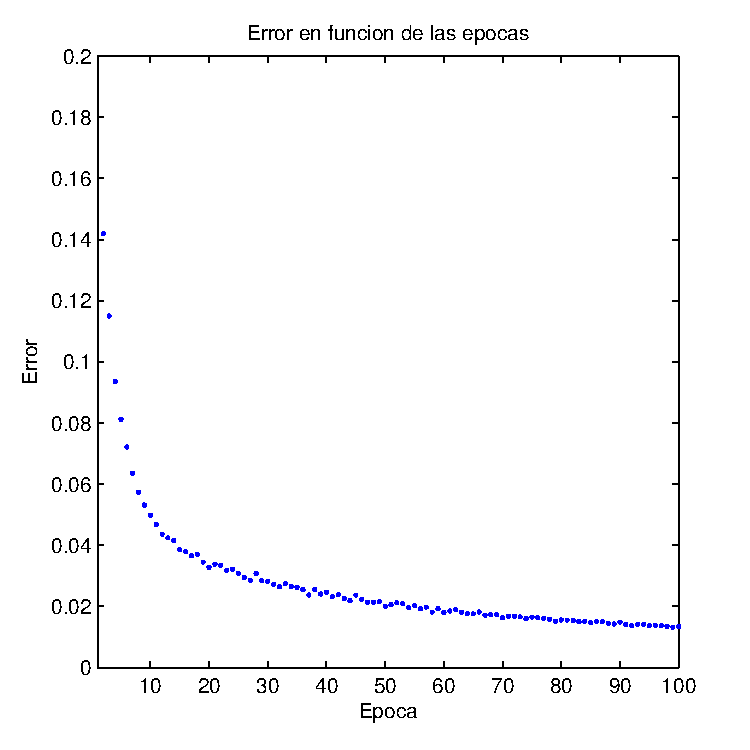
\includegraphics[width=\textwidth]{graficos/error_fold1_15_binary_100_02.pdf}
                \caption{Usando 15 neuronas.}
                \label{fig:d1-f1-02-n15}
        \end{subfigure}
        \begin{subfigure}[b]{0.32\textwidth}
                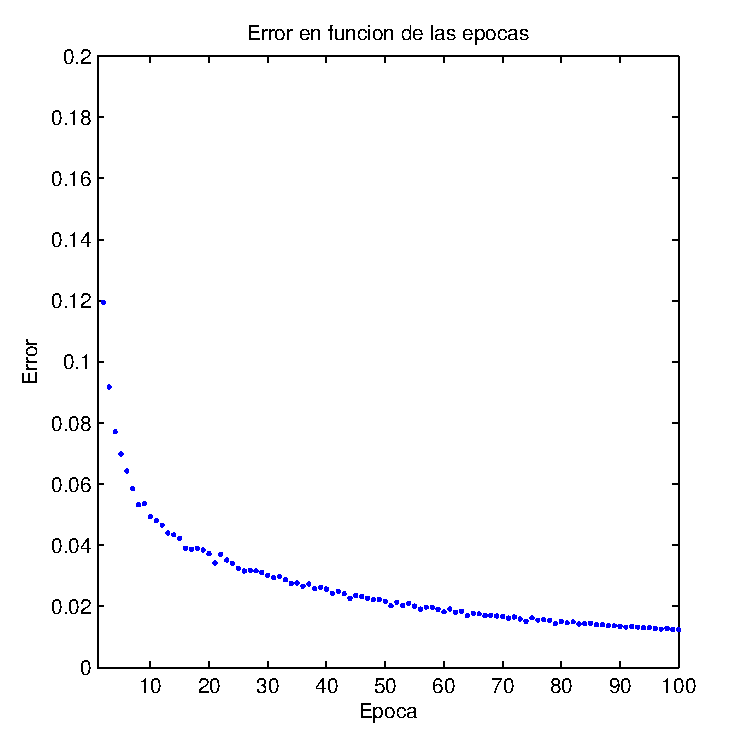
\includegraphics[width=\textwidth]{graficos/error_fold1_20_binary_100_02.pdf}
                \caption{Usando 20 neuronas.}
                \label{fig:d1-f1-02-n20}
        \end{subfigure}
        \begin{subfigure}[b]{0.32\textwidth}
                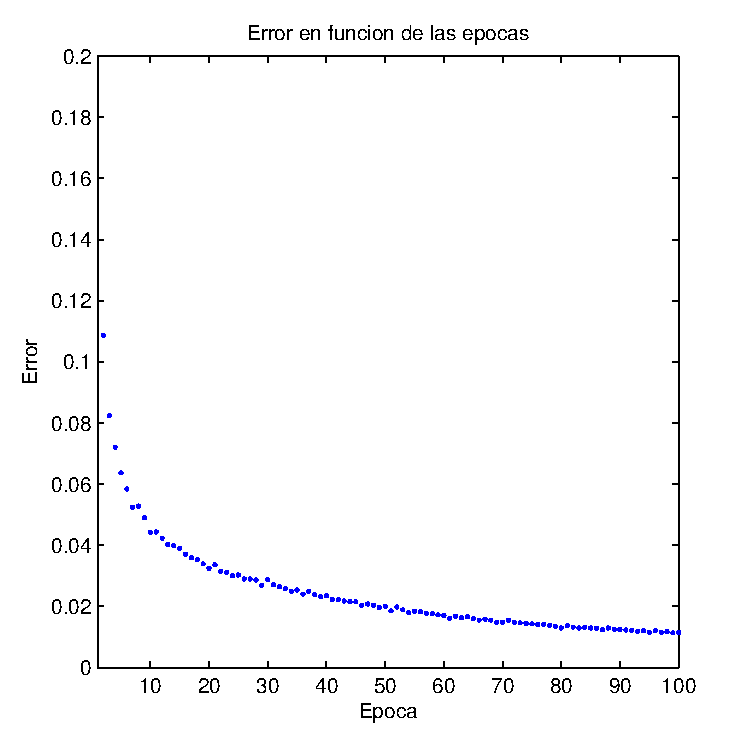
\includegraphics[width=\textwidth]{graficos/error_fold1_25_binary_100_02.pdf}
                \caption{Usando 25 neuronas.}
                \label{fig:d1-f1-02-n25}
        \end{subfigure}
        
        \caption{Error durante el entrenamiento en el fold 1 del problema 1 usando una sola capa oculta y $\gamma=0.2$.}\label{fig:p1-f1-gamma02}
    \end{figure}    

    \begin{figure}[H]
        \centering
        \begin{subfigure}[b]{0.32\textwidth}
                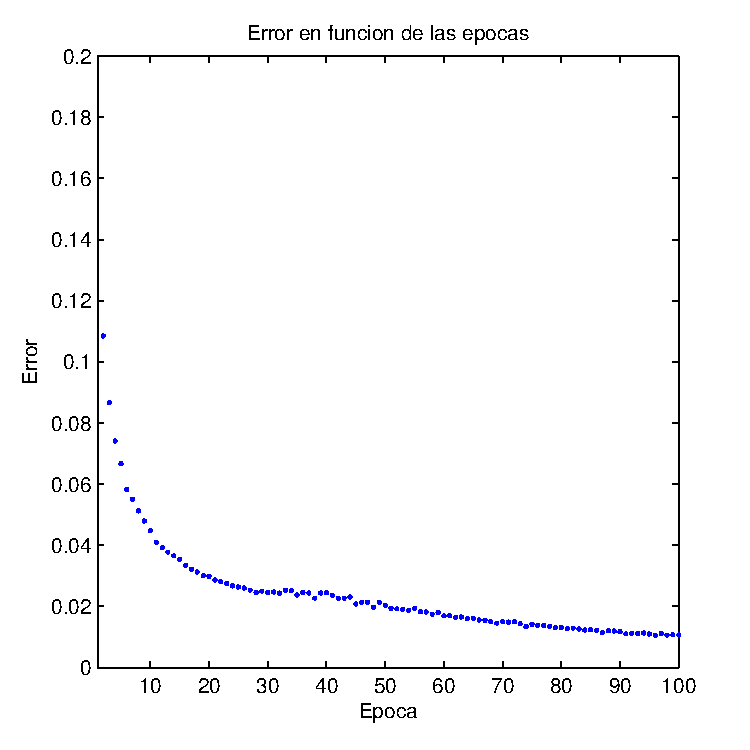
\includegraphics[width=\textwidth]{graficos/error_fold1_15_binary_100_03.pdf}
                \caption{Usando 15 neuronas.}
                \label{fig:d1-f1-03-n15}
        \end{subfigure}
        \begin{subfigure}[b]{0.32\textwidth}
                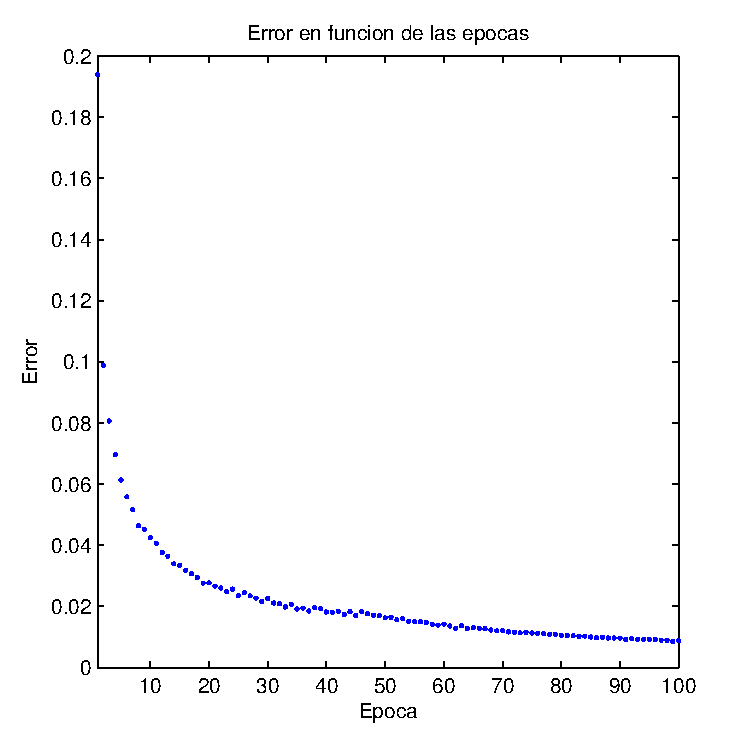
\includegraphics[width=\textwidth]{graficos/error_fold1_20_binary_100_03.pdf}
                \caption{Usando 20 neuronas.}
                \label{fig:d1-f1-03-n20}
        \end{subfigure}
        \begin{subfigure}[b]{0.32\textwidth}
                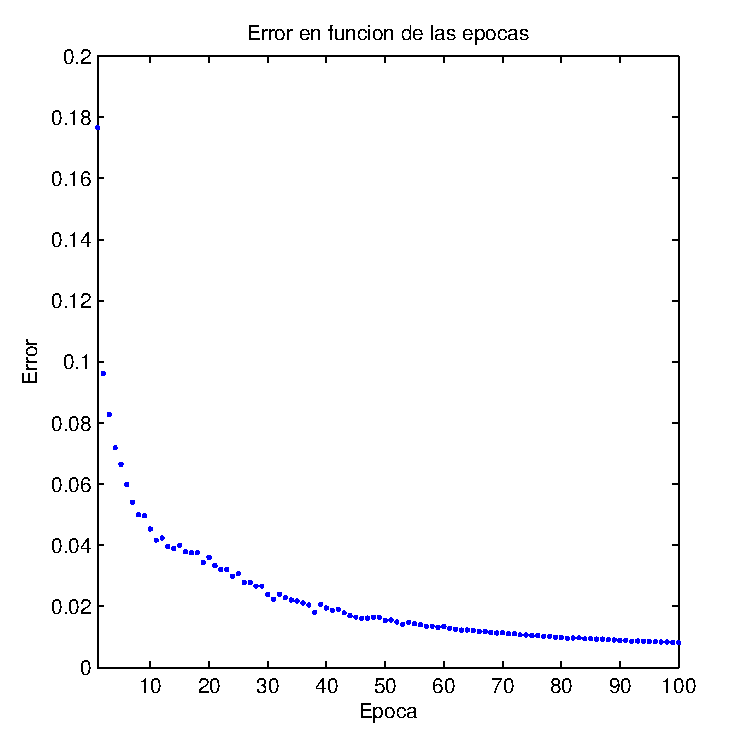
\includegraphics[width=\textwidth]{graficos/error_fold1_25_binary_100_03.pdf}
                \caption{Usando 25 neuronas.}
                \label{fig:d1-f1-03-n25}
        \end{subfigure}
        
        \caption{Error durante el entrenamiento en el fold 1 del problema 1 usando una sola capa oculta y $\gamma=0.3$.}\label{fig:p1-f1-gamma03}
    \end{figure}    
    
    \begin{figure}[H]
        \centering
        \begin{subfigure}[b]{0.32\textwidth}
                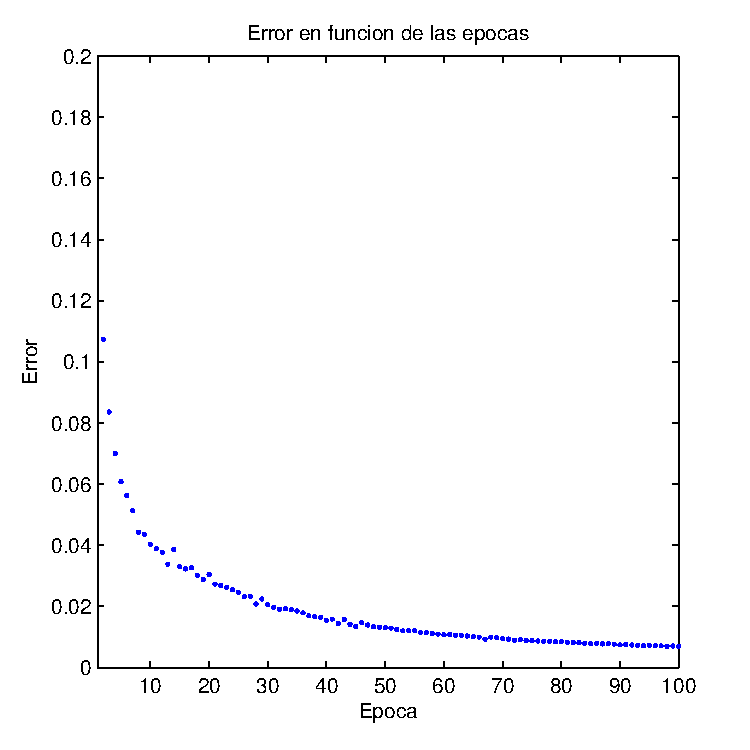
\includegraphics[width=\textwidth]{graficos/error_fold1_15_binary_100_04.pdf}
                \caption{Usando 15 neuronas.}
                \label{fig:d1-f1-04-n15}
        \end{subfigure}
        \begin{subfigure}[b]{0.32\textwidth}
                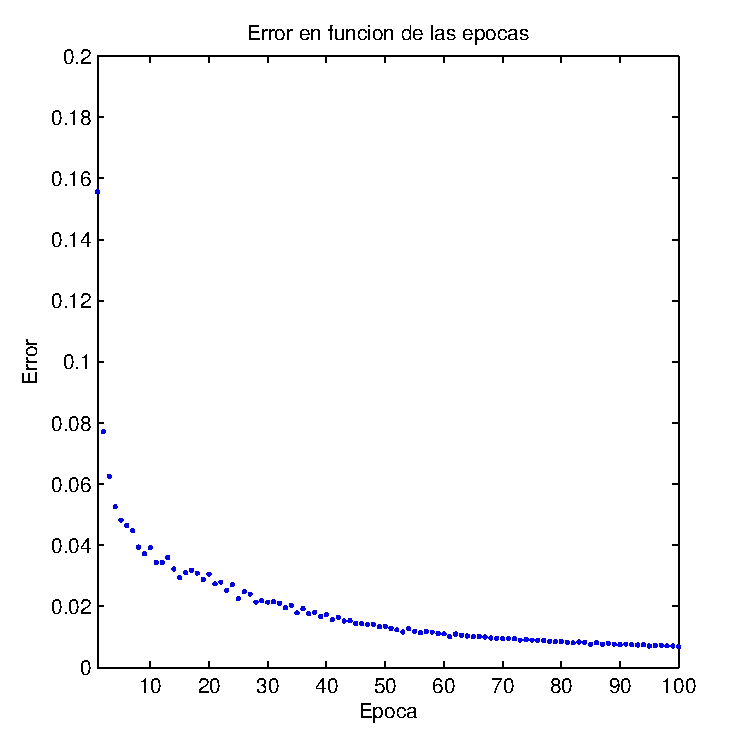
\includegraphics[width=\textwidth]{graficos/error_fold1_20_binary_100_04.pdf}
                \caption{Usando 20 neuronas.}
                \label{fig:d1-f1-04-n20}
        \end{subfigure}
        \begin{subfigure}[b]{0.32\textwidth}
                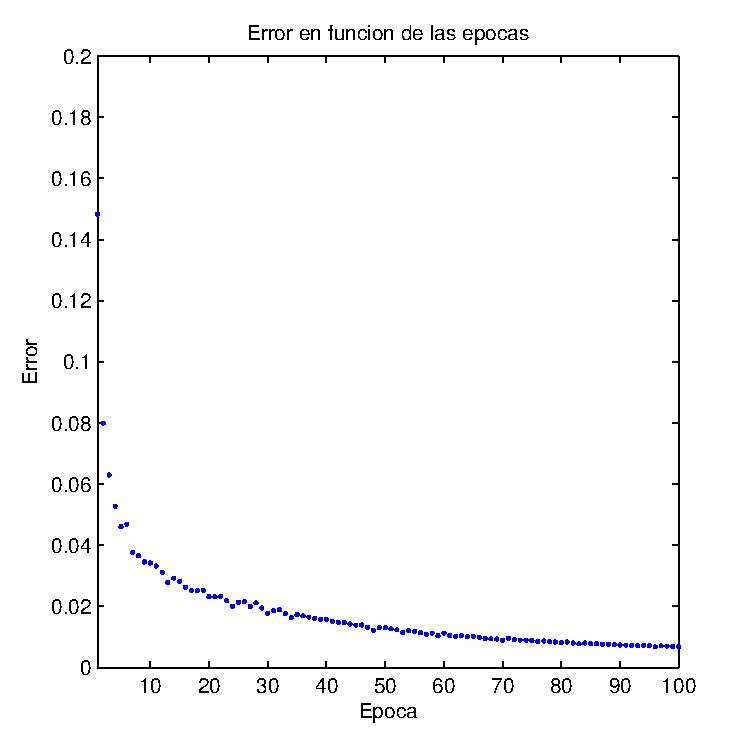
\includegraphics[width=\textwidth]{graficos/error_fold1_25_binary_100_04.pdf}
                \caption{Usando 25 neuronas.}
                \label{fig:d1-f1-04-n25}
        \end{subfigure}
        
        \caption{Error durante el entrenamiento en el fold 1 del problema 1 usando una sola capa oculta y $\gamma=0.4$.}\label{fig:p1-f1-gamma04}
    \end{figure}    

    \begin{figure}[H]
        \centering
        \begin{subfigure}[b]{0.32\textwidth}
                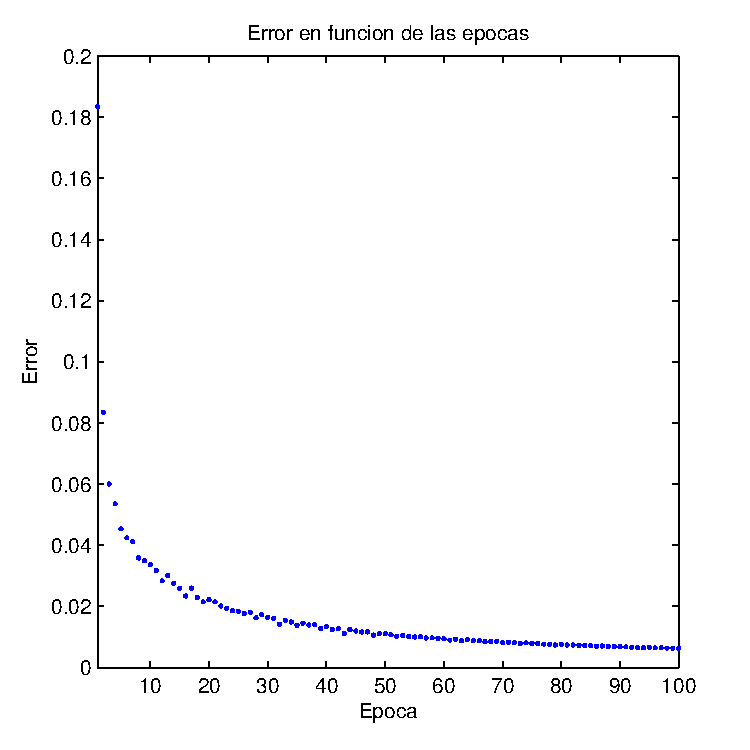
\includegraphics[width=\textwidth]{graficos/error_fold1_15_binary_100_05.pdf}
                \caption{Usando 15 neuronas.}
                \label{fig:d1-f1-05-n15}
        \end{subfigure}
        \begin{subfigure}[b]{0.32\textwidth}
                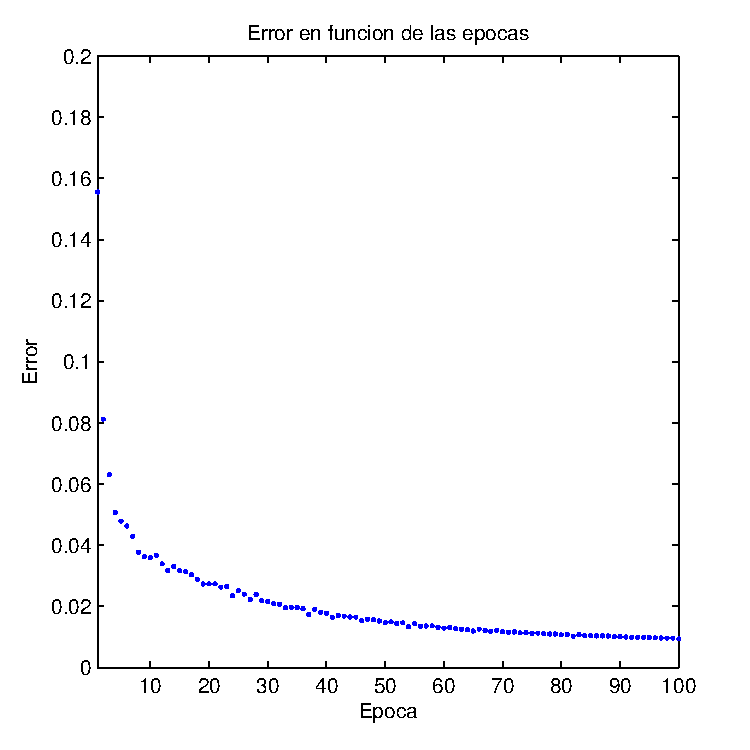
\includegraphics[width=\textwidth]{graficos/error_fold1_20_binary_100_05.pdf}
                \caption{Usando 20 neuronas.}
                \label{fig:d1-f1-05-n20}
        \end{subfigure}
        \begin{subfigure}[b]{0.32\textwidth}
                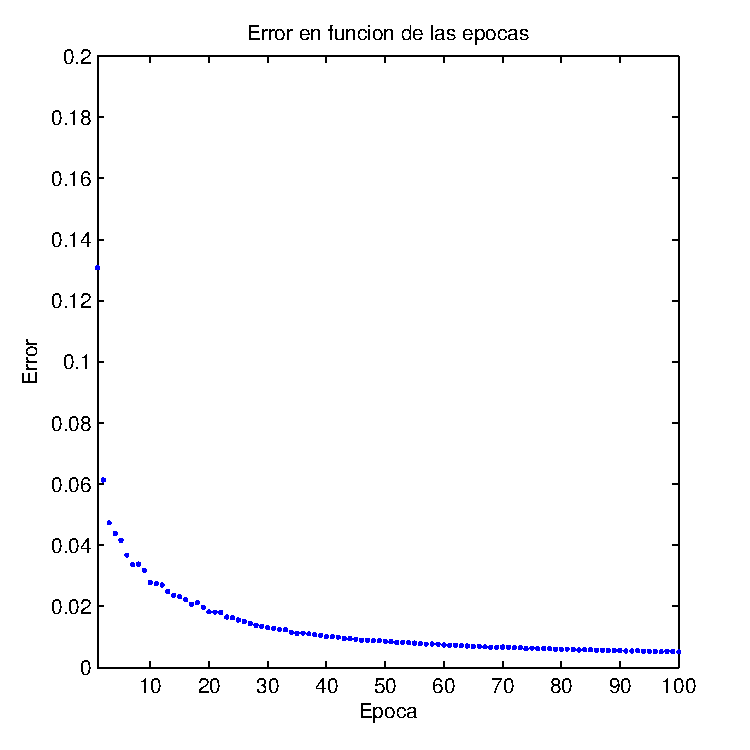
\includegraphics[width=\textwidth]{graficos/error_fold1_25_binary_100_05.pdf}
                \caption{Usando 25 neuronas.}
                \label{fig:d1-f1-05-n25}
        \end{subfigure}
        
        \caption{Error durante el entrenamiento en el fold 1 del problema 1 usando una sola capa oculta y $\gamma=0.5$.}\label{fig:p1-f1-gamma05}
    \end{figure}    
    
    
    
    \begin{table}
      \begin{center}
	\begin{tabular}{|c|c|c|c|}
	\hline
	& 15 neuronas & 20 neuronas & 25 neuronas \\ 
	\hline
	$\gamma=0.1$ & 0.041432 & 0.043057 & 0.034287 \\
	\hline
	$\gamma=0.2$ & 0.039383 & 0.028796 & 0.045242 \\
	\hline
	$\gamma=0.3$ & 0.034535 & 0.033598 & 0.02312 \\
	\hline
	$\gamma=0.4$ & 0.034545 & 0.037957 & 0.036029 \\
	\hline     
	$\gamma=0.5$ & 0.038391 & 0.03332 & 0.025975 \\
	\hline      
	\end{tabular}
	\caption{Error de validación luego de 100 iteraciones en el fold 1 del problema 1.}
	\label{tab:error-d1-f1}
      \end{center}
    \end{table}
    
    
    \subsection{Problema 2}
    
      A continuación (Figura \ref{fig:p2-f2-gamma01}) mostramos los errores de entrenamiento en función de la época al entrenar las redes con diversas cantidades de neuronas en el fold 2 aunque comportamientos similares fueron observados en el resto de los folds. Se puede observar cómo la cantidad de neuronas en la capa oculta juega un papel esencial en el error obtenido. Dado que cuanto mayor es el número de neuronas, mejores resultados obtenemos, decidimos analizar los resultados usando 16, 17, 18, 19 y 20 neuronas, mostrados en la Figura \ref{fig:p2-f2-gamma01-segundaParte}.
      
    \begin{figure}[H]
        \centering
        \begin{subfigure}[b]{0.32\textwidth}
                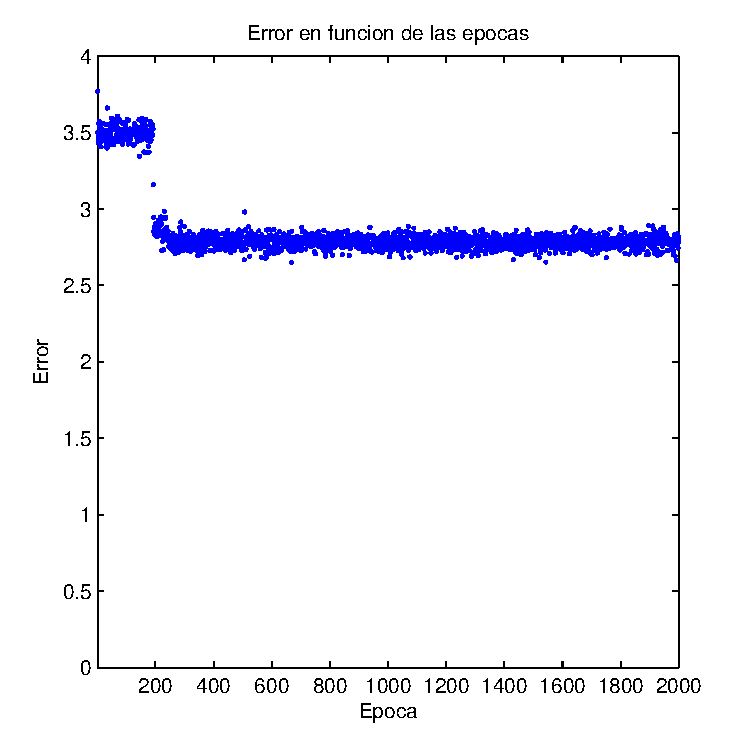
\includegraphics[width=\textwidth]{graficos/error_fold2_2_binary-regresion_2000_01.pdf}
                \caption{Usando 2 neuronas.}
                \label{fig:d2-f2-2k-01-n2}
        \end{subfigure}
        \begin{subfigure}[b]{0.32\textwidth}
                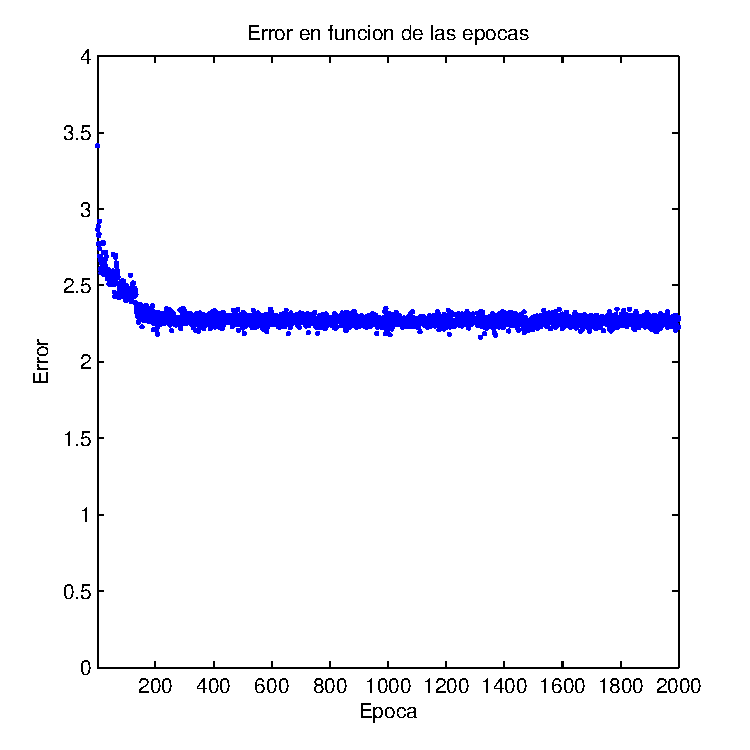
\includegraphics[width=\textwidth]{graficos/error_fold2_4_binary-regresion_2000_01.pdf}
                \caption{Usando 4 neuronas.}
                \label{fig:d2-f2-2k-01-n4}
        \end{subfigure}
        \begin{subfigure}[b]{0.32\textwidth}
                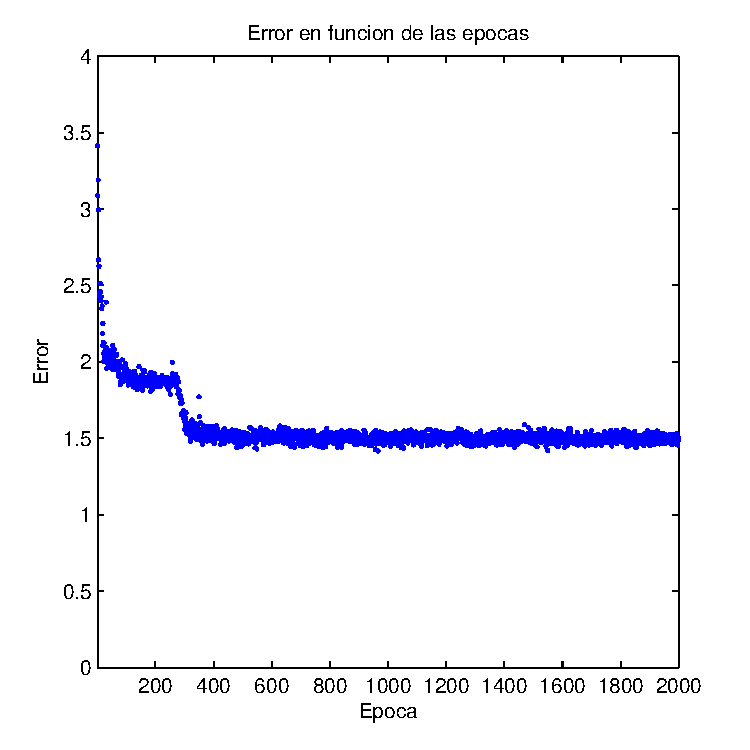
\includegraphics[width=\textwidth]{graficos/error_fold2_6_binary-regresion_2000_01.pdf}
                \caption{Usando 6 neuronas.}
                \label{fig:d2-f2-2k-01-n6}
        \end{subfigure}
        
        \begin{subfigure}[b]{0.32\textwidth}
                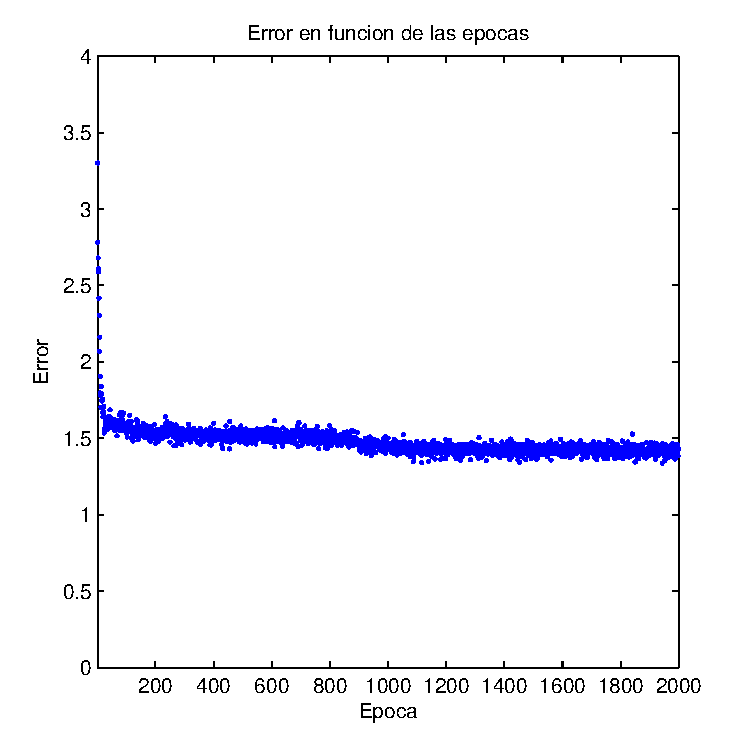
\includegraphics[width=\textwidth]{graficos/error_fold2_8_binary-regresion_2000_01.pdf}
                \caption{Usando 8 neuronas.}
                \label{fig:d2-f2-2k-01-n8}
        \end{subfigure}
        \begin{subfigure}[b]{0.32\textwidth}
                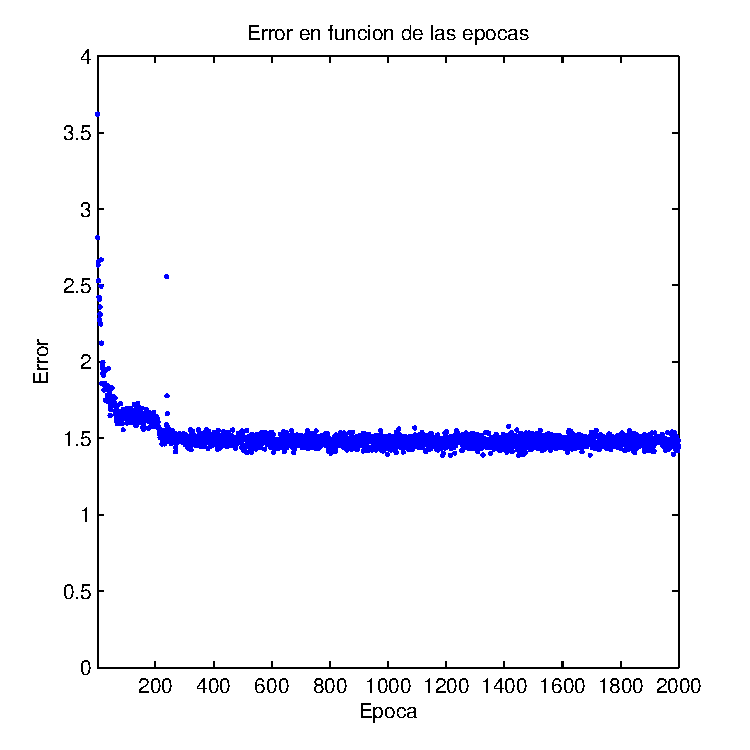
\includegraphics[width=\textwidth]{graficos/error_fold2_10_binary-regresion_2000_01.pdf}
                \caption{Usando 10 neuronas.}
                \label{fig:d2-f2-2k-01-n10}
        \end{subfigure}
        \begin{subfigure}[b]{0.32\textwidth}
                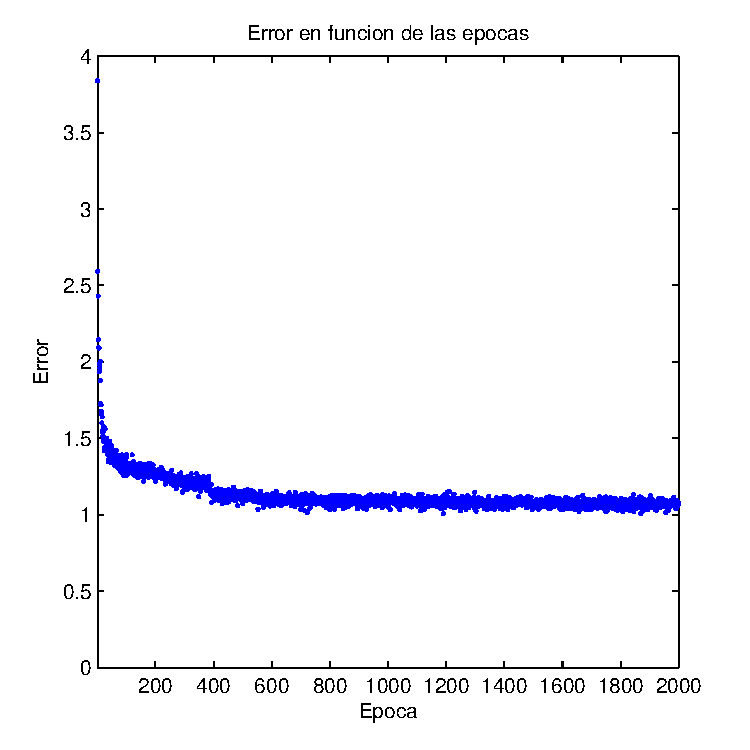
\includegraphics[width=\textwidth]{graficos/error_fold2_12_binary-regresion_2000_01.pdf}
                \caption{Usando 12 neuronas.}
                \label{fig:d2-f2-2k-01-n12}
        \end{subfigure}
        
        \begin{subfigure}[b]{0.32\textwidth}
                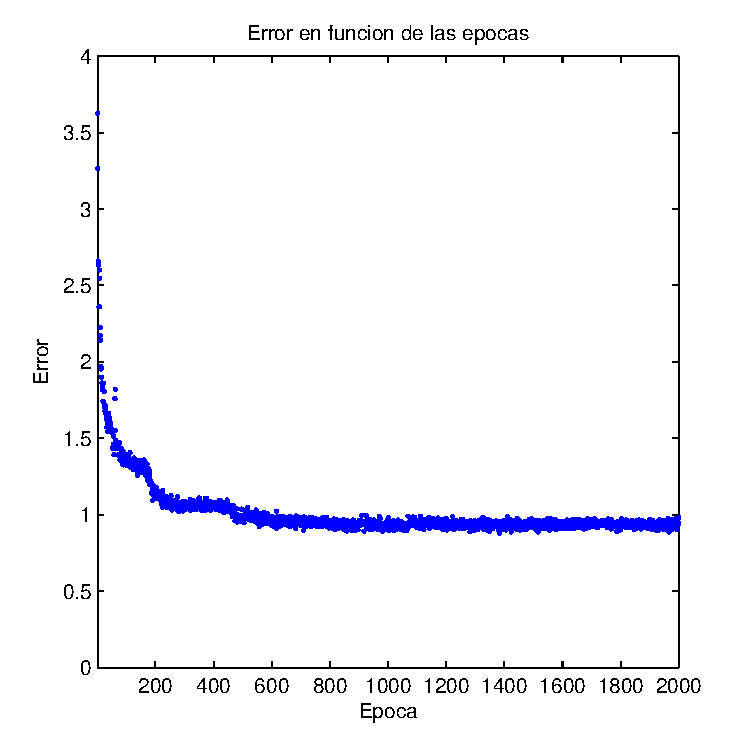
\includegraphics[width=\textwidth]{graficos/error_fold2_14_binary-regresion_2000_01.pdf}
                \caption{Usando 14 neuronas.}
                \label{fig:d2-f2-2k-01-n14}
        \end{subfigure}
        
        \caption{Error durante el entrenamiento en el fold 2 del problema 2 usando una sola capa oculta y $\gamma=0.1$.}\label{fig:p2-f2-gamma01}
    \end{figure}
    
    
    \begin{figure}[H]
        \centering
        \begin{subfigure}[b]{0.32\textwidth}
                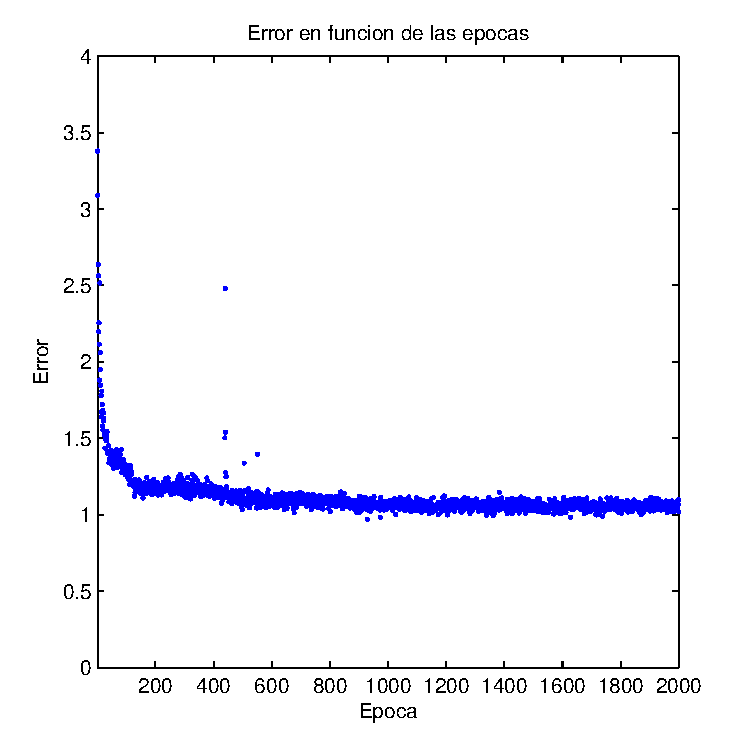
\includegraphics[width=\textwidth]{graficos/error_fold2_16_binary-regresion_2000_01.pdf}
                \caption{Usando 16 neuronas.}
                \label{fig:d2-f2-2k-01-n16}
        \end{subfigure}
        \begin{subfigure}[b]{0.32\textwidth}
                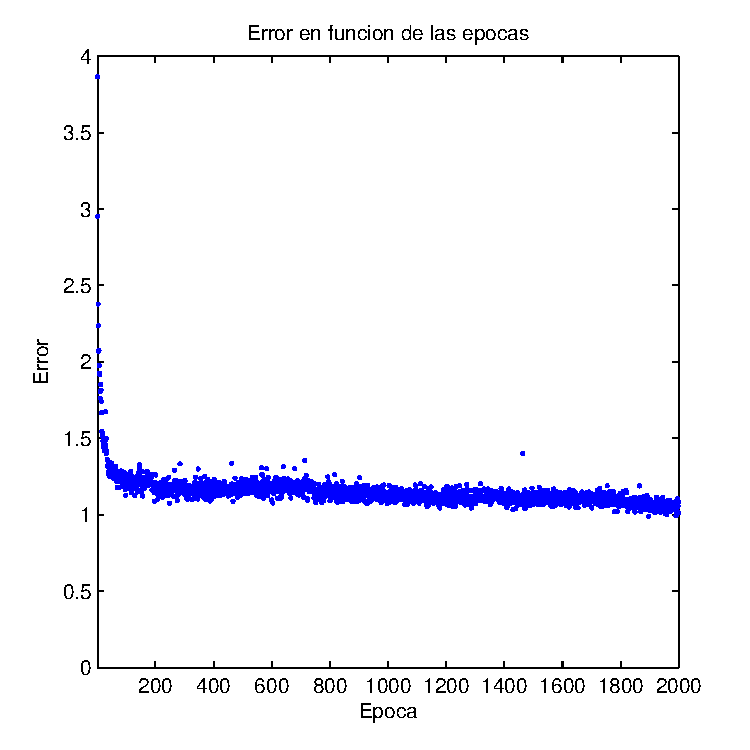
\includegraphics[width=\textwidth]{graficos/error_fold2_17_binary-regresion_2000_01.pdf}
                \caption{Usando 17 neuronas.}
                \label{fig:d2-f2-2k-01-n17}
        \end{subfigure}
        \begin{subfigure}[b]{0.32\textwidth}
                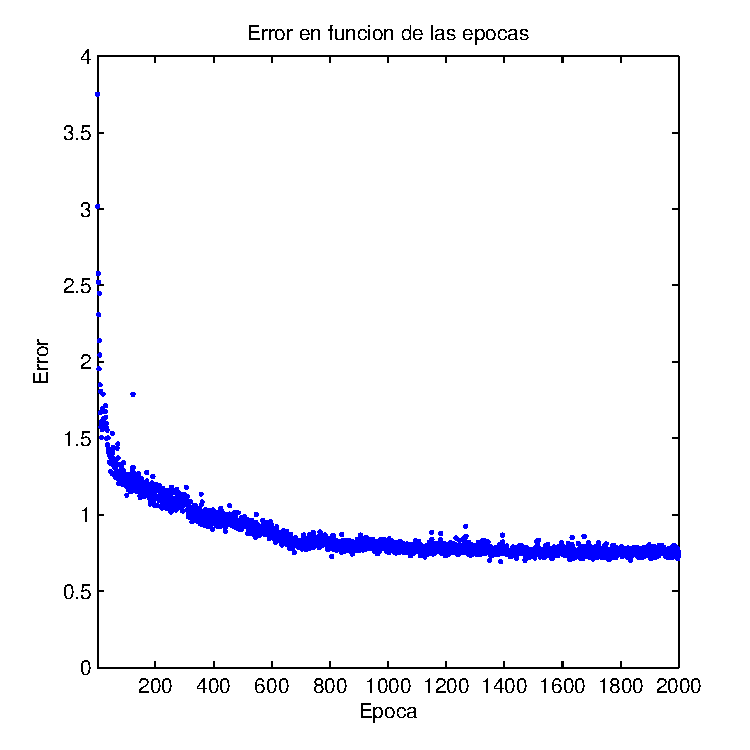
\includegraphics[width=\textwidth]{graficos/error_fold2_18_binary-regresion_2000_01.pdf}
                \caption{Usando 18 neuronas.}
                \label{fig:d2-f2-2k-01-n18}
        \end{subfigure}
        
        \begin{subfigure}[b]{0.32\textwidth}
                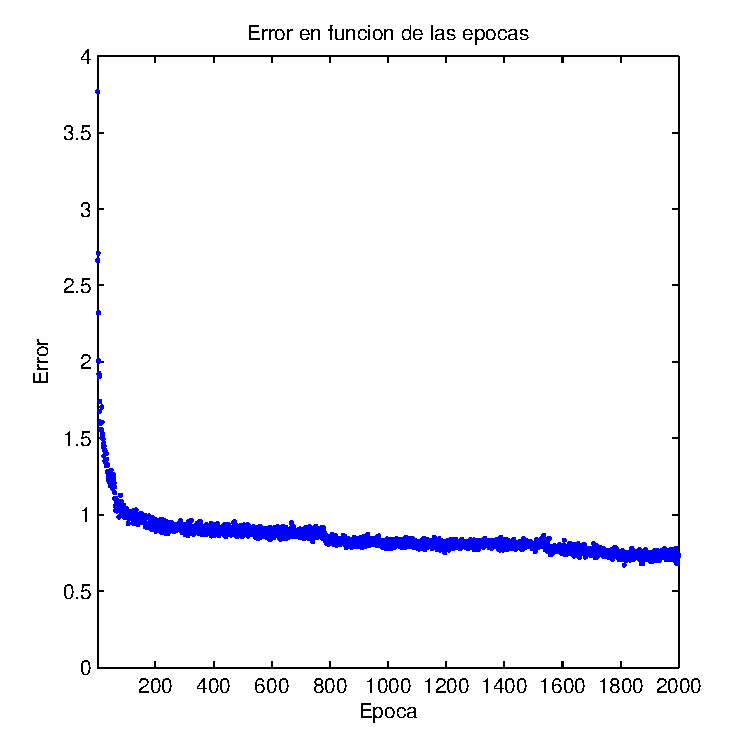
\includegraphics[width=\textwidth]{graficos/error_fold2_19_binary-regresion_2000_01.pdf}
                \caption{Usando 19 neuronas.}
                \label{fig:d2-f2-2k-01-n19}
        \end{subfigure}
        \begin{subfigure}[b]{0.32\textwidth}
                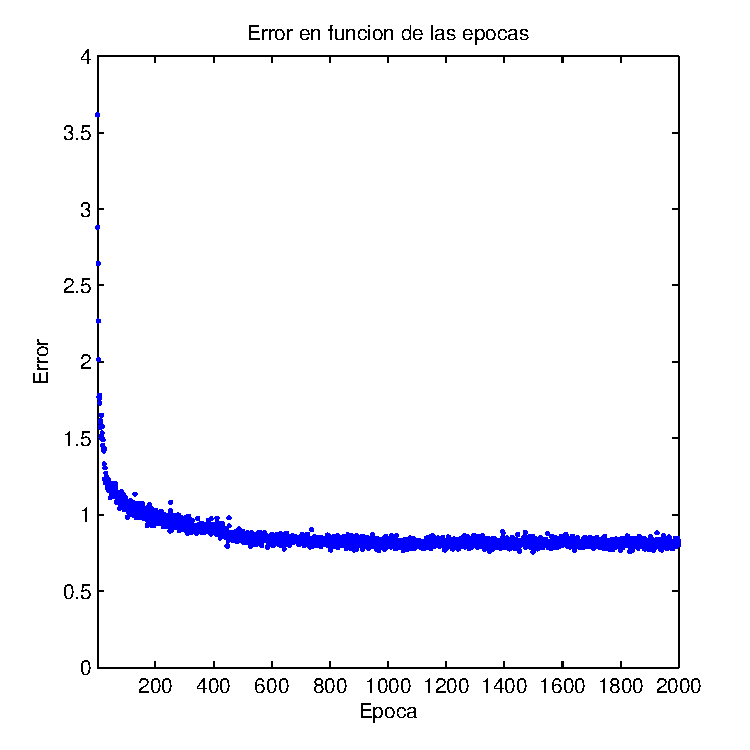
\includegraphics[width=\textwidth]{graficos/error_fold2_20_binary-regresion_2000_01.pdf}
                \caption{Usando 20 neuronas.}
                \label{fig:d2-f2-2k-01-n20}
        \end{subfigure}
        
        \caption{Error durante el entrenamiento en el fold 2 del problema 2 usando una sola capa oculta y $\gamma=0.1$ segunda parte. Error en el conjunto de test (promedio entre los cuatro folds): 1,758475, 1,926875, 1,82305, 1,4711275 y 1,38239 respectivamente.}\label{fig:p2-f2-gamma01-segundaParte}
    \end{figure}
    
    
    Tomando los resultados de las Figuras \ref{fig:p2-f2-gamma01} y \ref{fig:p2-f2-gamma01-segundaParte} se puede ver que los errores (tanto en entrenamiento como en validaci\'on) m\'as bajos se obtienen usando 20 neuronas, además de un comportamiento estable por lo que decidimos no buscar configuraciones con más neuronas.
    
    Considerando esa arquitectura, decidimos analizar otros valores de learning rate a fin de observar si es posible converger más rápido. Los resultados se encuentran en la Figura \ref{fig:p2-f2-gammasVarios}.
    
    \begin{figure}[H]
        \centering
        \begin{subfigure}[b]{0.32\textwidth}
                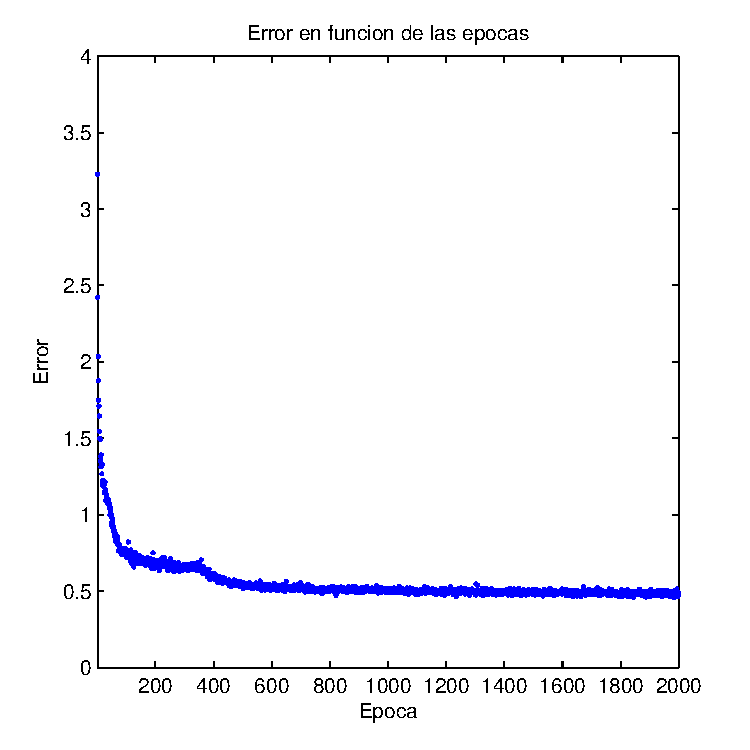
\includegraphics[width=\textwidth]{graficos/error_fold2_20_binary-regresion_2000_001.pdf}
                \caption{Con $\gamma=0.01$.}
                \label{fig:d2-f2-2k-001-n20}
        \end{subfigure}
        \begin{subfigure}[b]{0.32\textwidth}
                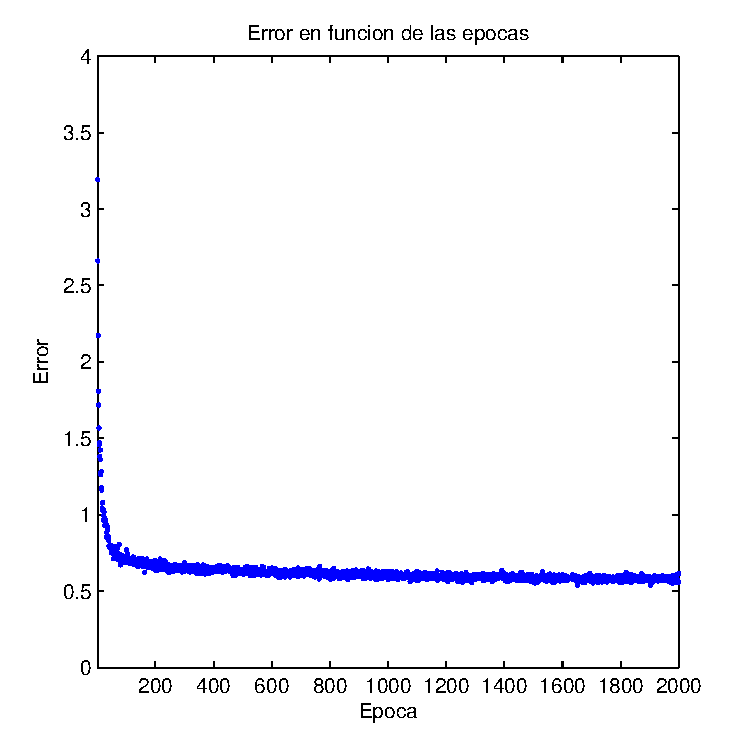
\includegraphics[width=\textwidth]{graficos/error_fold2_20_binary-regresion_2000_005.pdf}
                \caption{Con $\gamma=0.05$.}
                \label{fig:d2-f2-2k-005-n20}
        \end{subfigure}
        \begin{subfigure}[b]{0.32\textwidth}
                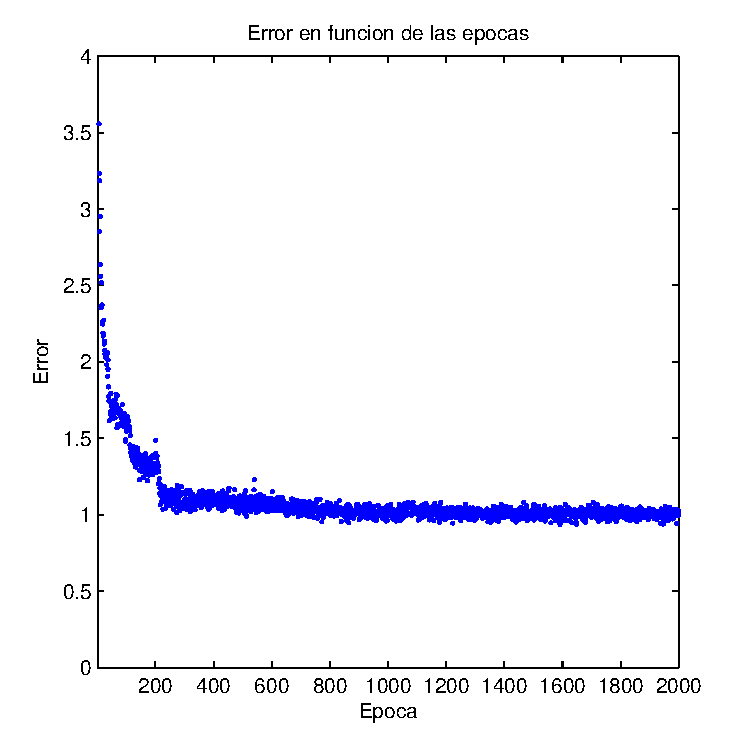
\includegraphics[width=\textwidth]{graficos/error_fold2_20_binary-regresion_2000_015.pdf}
                \caption{Con $\gamma=0.15$.}
                \label{fig:d2-f2-2k-015-n20}
        \end{subfigure}
        
        \caption{Error durante el entrenamiento en el fold 2 del problema 2 usando una sola capa oculta de 20 neuronas variando el valor de $\gamma$.}\label{fig:p2-f2-gammasVarios}
    \end{figure}
    
    
\end{document}